
%%%%%%%%%%%%%%%%%%%%%%%%%%%%%%%%%%%%%%%%%%%%%%%%%%%%%%%%%%%%%%%%%%%%%%%%%%%%%%%%%%%%%%%%%%%%%%%%%%%%%%%%%%%%%%%%%%%%%%%%%%%%%%%%%%%%%%%%%%%%%%%%%%%%%%%%%%%%%%%%%%%%
\chapter{How do I look at QTLs in Ondex?}
\label{cha:qtl}
%%%%%%%%%%%%%%%%%%%%%%%%%%%%%%%%%%%%%%%%%%%%%%%%%%%%%%%%%%%%%%%%%%%%%%%%%%%%%%%%%%
%Intro TO DO

\section*{Application case: Candidate genes for biomass traits}
\label{sec:k1}

As there is a need to understand plant architecture related to yield ({\it{e.g.}}, branching process),
we wish to identify genes controlling biomass production in willow (a second generation bioenergy crop). 
Even well-defined QTL may encompass many potential candidate genes (perhaps hundreds),
it is therefore difficult to objectively choose underlying candidate(s) that drive the phenotype.
We are developing means to support systematic analysis of QTL regions and to prioritise genes for experimental analyses.

The willow genome is not yet fully sequenced.
Poplar is the first tree with a fully sequenced genome.
It has 19 chromosomes, 45555 predicted genes (4 times larger than \textit{Arabidopsis's} genome).
Not much is known yet about the function of poplar genes.

We are using comparative genomics to compare poplar to \textit{Arabidopsis} to find linked references, expression patterns, pathways, plant hormones and ontologies
in order to link genes between the two.
The genome annotation pipeline integrates data together from UniProtKB, TAIR, Gramene, GO, GOA, TraitOnt, PlantOnt, Medline, AraCyc and Pfam.
(A workflow named biomass\_integrator\_workflow.xml is available under Tutorial\_files/Application\_cases for this data integration pipeline).
The methods used for this integration are based on sequence similarity, domain analysis and text mining as shown in Figure \ref{fig:poplar_annotation_pipeline}.
This allows us to achieve automatic function prediction with different levels of evidence.

\begin{figure}[H]
\centering
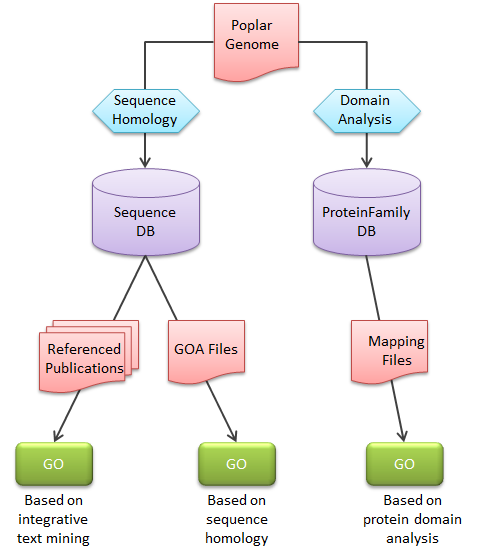
\includegraphics[scale=0.8]{images/Oct12/poplarkb_pipeline.png} 
\caption{Poplar annotation pipeline}
\label{fig:poplar_annotation_pipeline}
\end{figure}

This data integration in Ondex resulted in the metagraph shown in Figure \ref{fig:poplar_metagraph}.
(The data is available under Tutorial\_files/Application\_cases, the graph is named biomass\_knowledge\_base\_subset.oxl).
Inspection of the metagraph shows the genes and the QTLs enriched with positional information as well as
the proteins annotated with GO, EC, KEGG and publications based on comparative genomics and protein family analysis.
\begin{figure}[H]
\centering
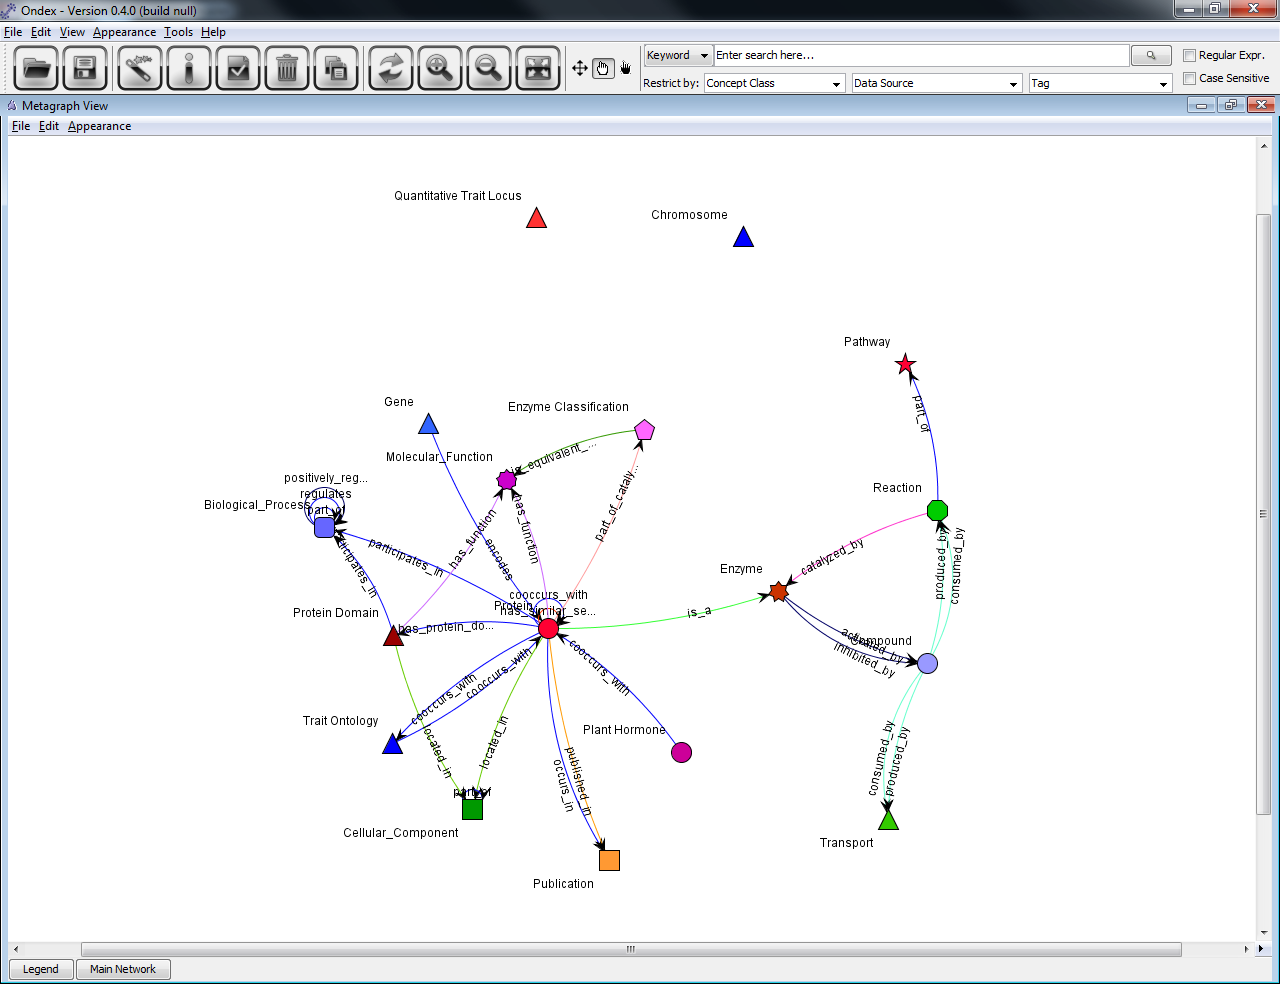
\includegraphics[scale=0.35]{images/Oct12/poplarkb_metagraph.png} 
\caption{Integrated poplar knowledge base subset}
\label{fig:poplar_metagraph}
\end{figure}

Had we opened the entire knowledge base, the Genomics layout would have enabled us to display chromosomes, genes and QTLs 
where chromosomal regions and QTLs can be selected (see Figure \ref{fig:poplar_genomic_view}).
\begin{figure}[H]
\centering
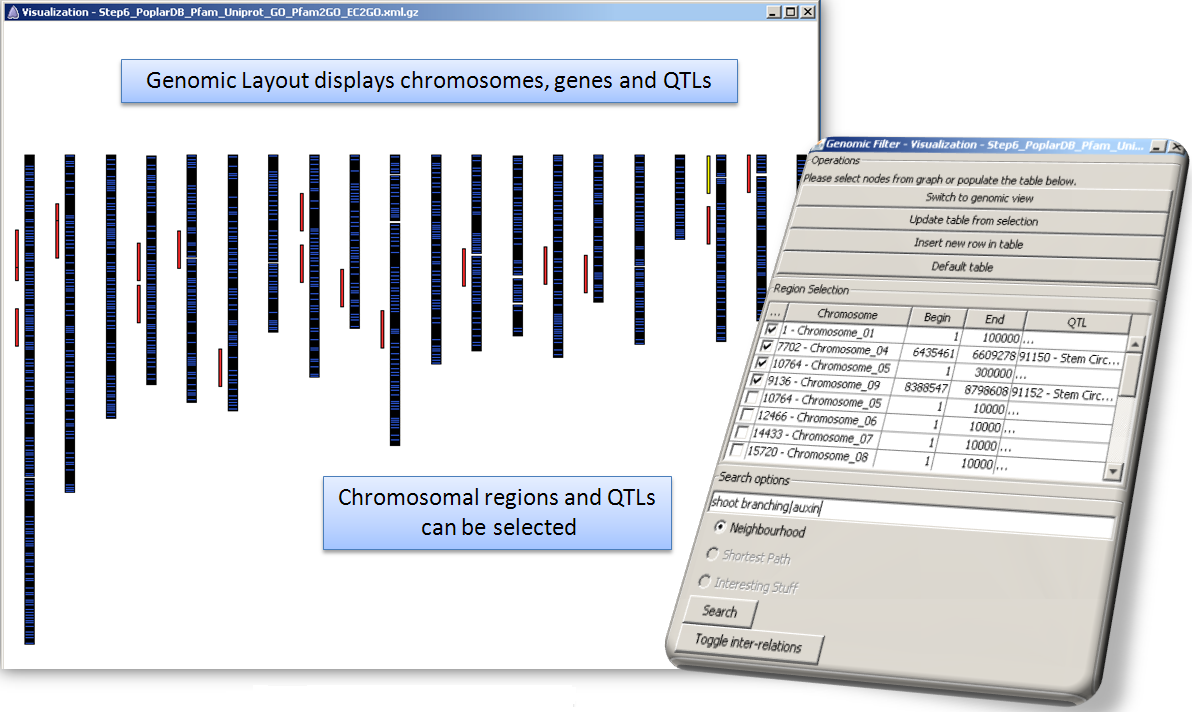
\includegraphics[scale=0.3]{images/Oct12/poplar_genomic_view.png} 
\caption{Genomics layout (Appearance menu) or Genomics filter (Tools -$>$ Filters -$>$ More -$>$ Genomics -$>$ Switch to genomic view)}
\label{fig:poplar_genomic_view}
\end{figure}

In many domains, we observe various phenotypes without being able to link them to genes which are responsible for them.
The aim of this application case is to identify genes controlling biomass production in willow (a second generation bioenergy crop). 
We are developing software which can support biologists and users to analyse QTLs
(genomic regions that help us narrow down potential candidate genes related to a phenotype).

We currently have two sources of data:
\begin{itemize}
\item QTL data is available for willow, however the willow genome is not yet fully sequenced
\item The poplar genome sequence is available and this species is very similar to willow, however very little is known about the function of poplar genes
\end{itemize}
A QTL can contain up to hundreds of genes. We therefore look to identify candidate genes that correspond to the observed phenotype.

In order to find similar sequences in other species that hold information on gene function,
we have undertaken a comparative genomics approach.
This allows us to gather data from free text (where information then needs to be automatically extracted), 
expression patterns, pathways, ontologies, {\it{etc.}}.

The genomic view in Ondex allows users to visualise chromosomes, genes and QTLs (in red).
The genomic filter allows users to select the regions they wish to study in more detail.
Users may also enter a few keywords in a search box.
Once they click on the search button, users are presented with the genes contained in the selected QTLs of interest (blue rectangles) and
these are linked to their corresponding proteins which, in turn, are linked to the orthologs found by the comparative analysis.
The orthologs are themselves linked to the information imported during the data integration.
The keywords previously entered in the search box are then used to highlight some concepts in the graph which contain them in their properties.
This feature is very useful as it allows users to directly focus on proteins that are relevant to their research work.
On the right-hand side of the visualisation window we can see some poplar proteins which are not linked to any extra information
because no orthologs were found.

Users can zoom into particular areas of the graph, they can also select a ``hot'' candidate and look at its neighbourhood
(using the neighbourhood filter).

Here are examples of combinations of steps that can be used to analyse the data where our trait of interest is ``shoot branching'' 
or the number of axillary branches:
\begin{itemize}
\item Load Tutorial\_files/Application\_cases/biomass\_knowledge\_base\_subset.oxl
\item Launch the Genomics filter (Tools -$>$ Filters -$>$ More -$>$ Genomics)
\item Select QTL ``No. axillary branches'' on the first line (chromosome 1).
Start and end of the QTL get filled in automatically this way. Untick the second line offered. 
\item Enter ``auxin'' in search options
\item Click on ``Search Region'' (see results in Figure \ref{fig:poplarkb_search_region})
\item Now select chromosome 4 as well with the same QTL
\item Click on ``Search Region'' (see results in Figure \ref{fig:poplarkb_search_region_2})
\item Click ``Show/Hide unrelated genes'' to make visible/invisible genes that are not linked to any keyword related concepts
\item After applying the Gem layout and adding labels, we get Figure \ref{fig:poplarkb_hide_unrelated_genes}
\end{itemize}

\begin{figure}[H]
\centering
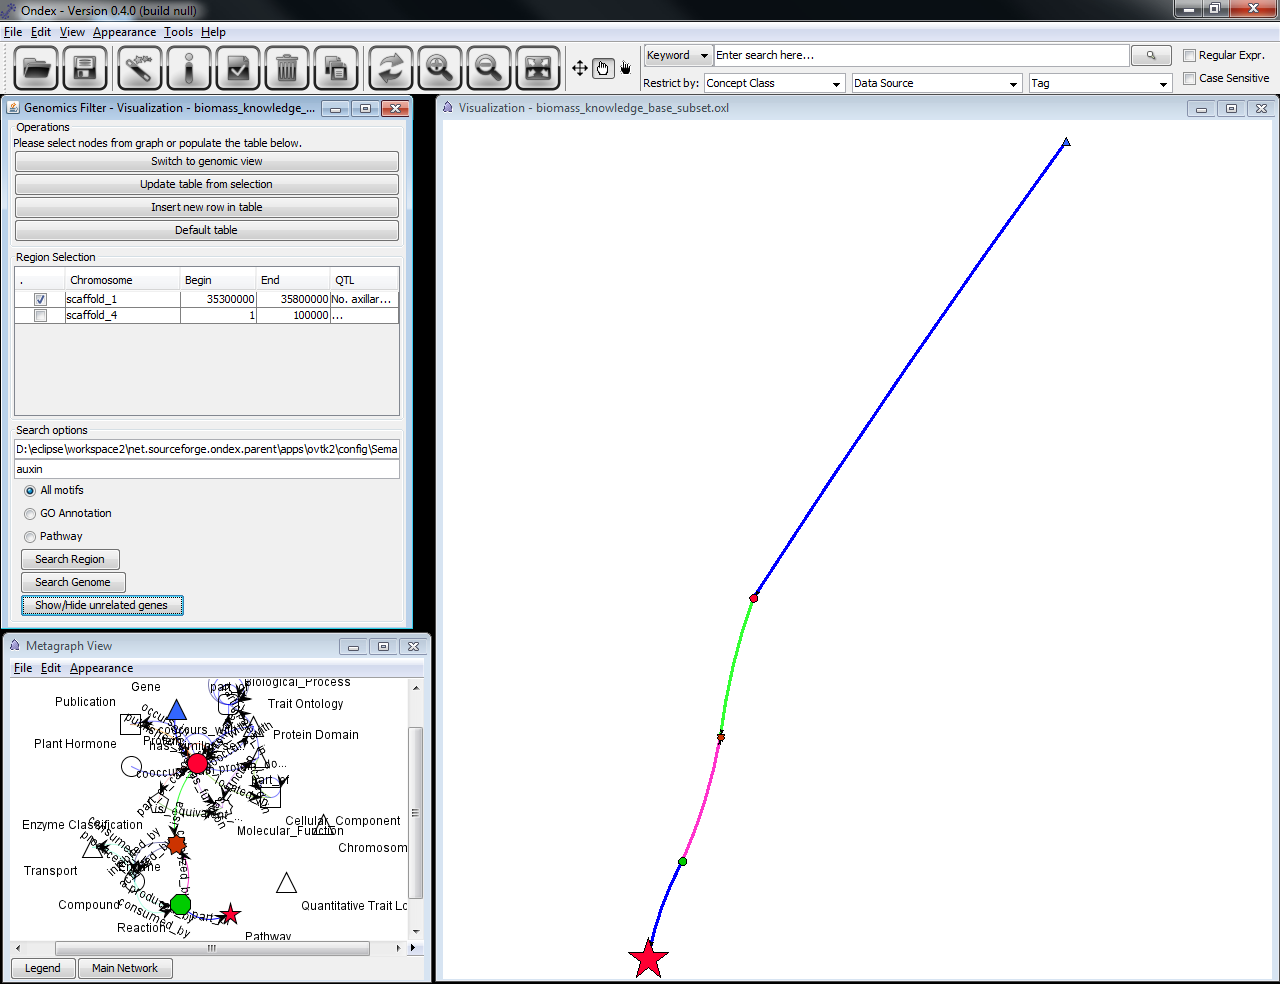
\includegraphics[scale=0.35]{images/Oct12/poplarkb_search_region.png} 
\caption{Search Region function in the Genomics Filter}
\label{fig:poplarkb_search_region}
\end{figure}

\begin{figure}[H]
\centering
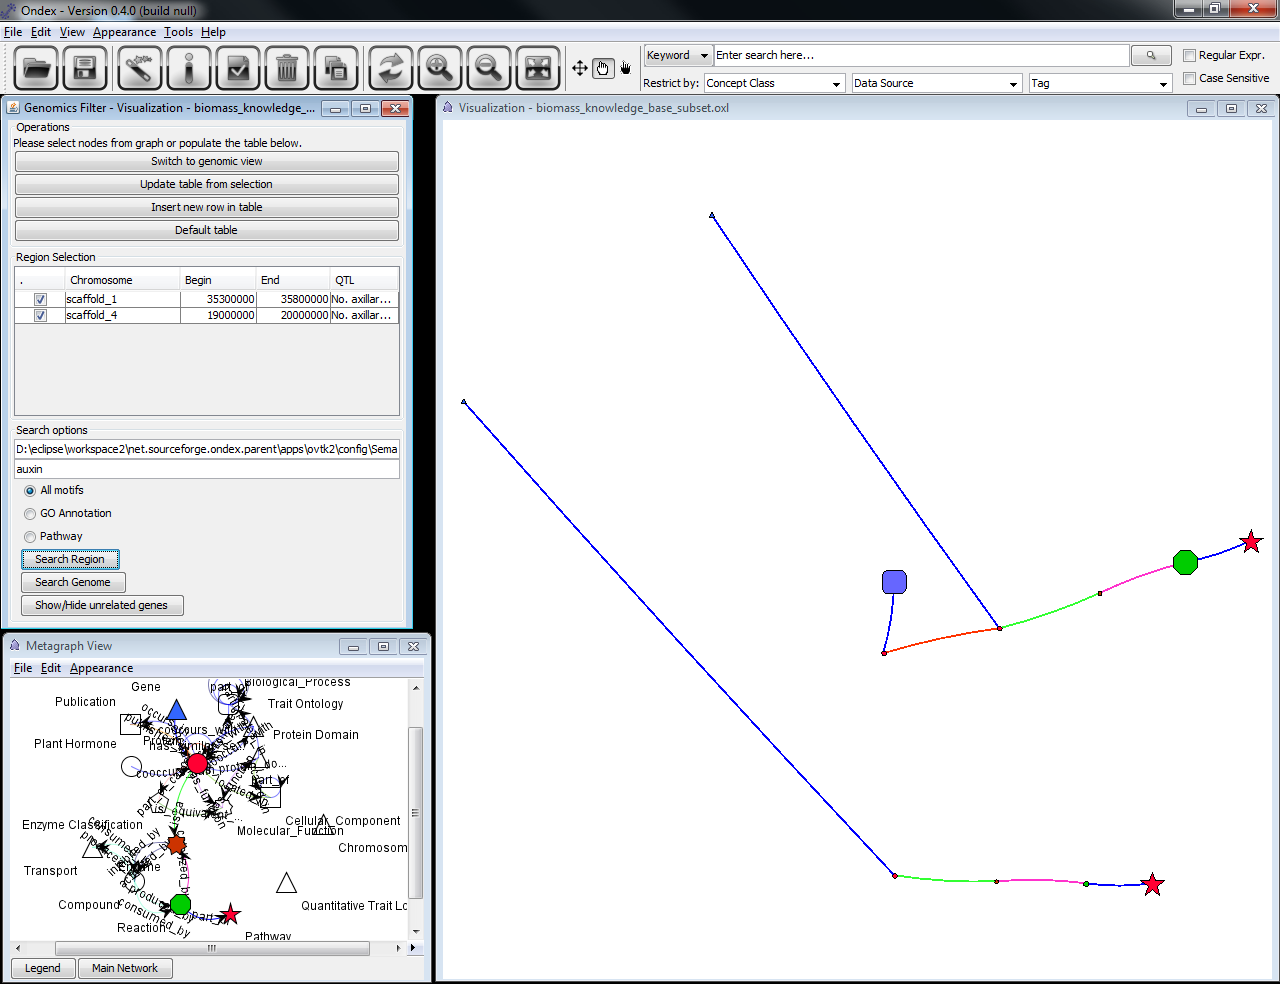
\includegraphics[scale=0.35]{images/Oct12/poplarkb_search_region_2.png} 
\caption{Search Region function in the Genomics Filter with both chromosomes selected}
\label{fig:poplarkb_search_region_2}
\end{figure}


\begin{figure}[H]
\centering
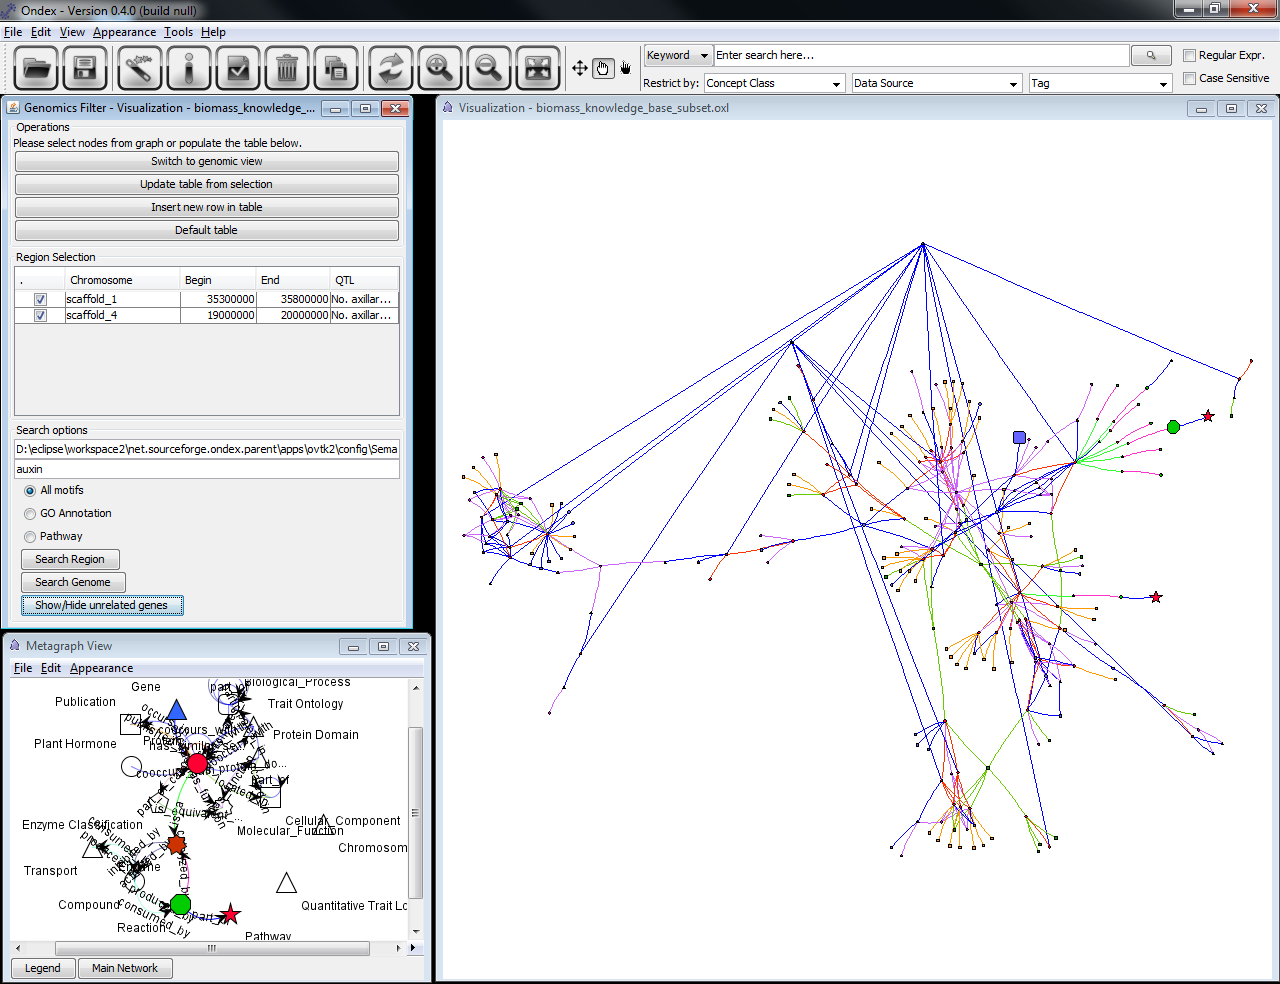
\includegraphics[scale=0.35]{images/Oct12/poplarkb_hide_unrelated_genes.png} 
\caption{Show/Hide unrelated genes function in the Genomics Filter}
\label{fig:poplarkb_hide_unrelated_genes}
\end{figure}

Each QTL has a gene which encodes an enzyme that is involved in an auxin related pathway.
Pathway view can connect genes of different QTL and explain phylogenetic traits.
